\begin{surferPage}[Octica de Chmutov]{A \'Octica de Chmutov}
    Uma caracter\'istica atraente da \'octica de Chmutov $\text{Chm}_{d}, \ d=8,$
    \'e a sua simetria, que pode tamb\'em ser identificada na sua equa\c c\~ao:
    \[\text{Chm}_{d}\colon T_d(x) + T_d(y) + T_d(z) + 1 = 0,\]
     onde $T_d$ \'e o  polin\'omio de Tchebychevl (imagem \`a esquerda).
    A curva $T_8(x)+T_8(y)=0$ est\'a representada \`a direita:
    
     \begin{center}
      \begin{tabular}{c@{\quad}c}
        \begin{tabular}{c}
          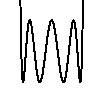
\includegraphics[height=1.75cm]{./../../common/images/Tcheb_008.pdf}
        \end{tabular}    
        &
        \begin{tabular}{c}
          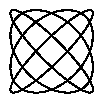
\includegraphics[height=1.75cm]{./../../common/images/Tcheb_2d_008.pdf}
        \end{tabular}    
      \end{tabular}
    \end{center}
    \vspace{-0.3cm}
    O caminho a seguir desde estas imagens at\'e \`a forma da superf\'icie no quadro interativo n\~ao \'e muito longo.


Essas equa\c c\~oes foram apresentadas por S.V.\ Chmutov no in\'icio dos anos 80.
    Naquela \'epoca, elas constitu\'iam o recorde mundial para $\mu(d)$ para a maioria dos $d$.
    Na d\'ecada de 90, Chmutov melhorou o seu pr\'oprio recorde e, em 2005, S.Breske,
    O.~Labs e D.~van~Straten adaptaram esta constru\c c\~ao para superf\'icies reais com apenas singularidades reais.
\end{surferPage}
